\begin{figure}[htbp]
    \centering
    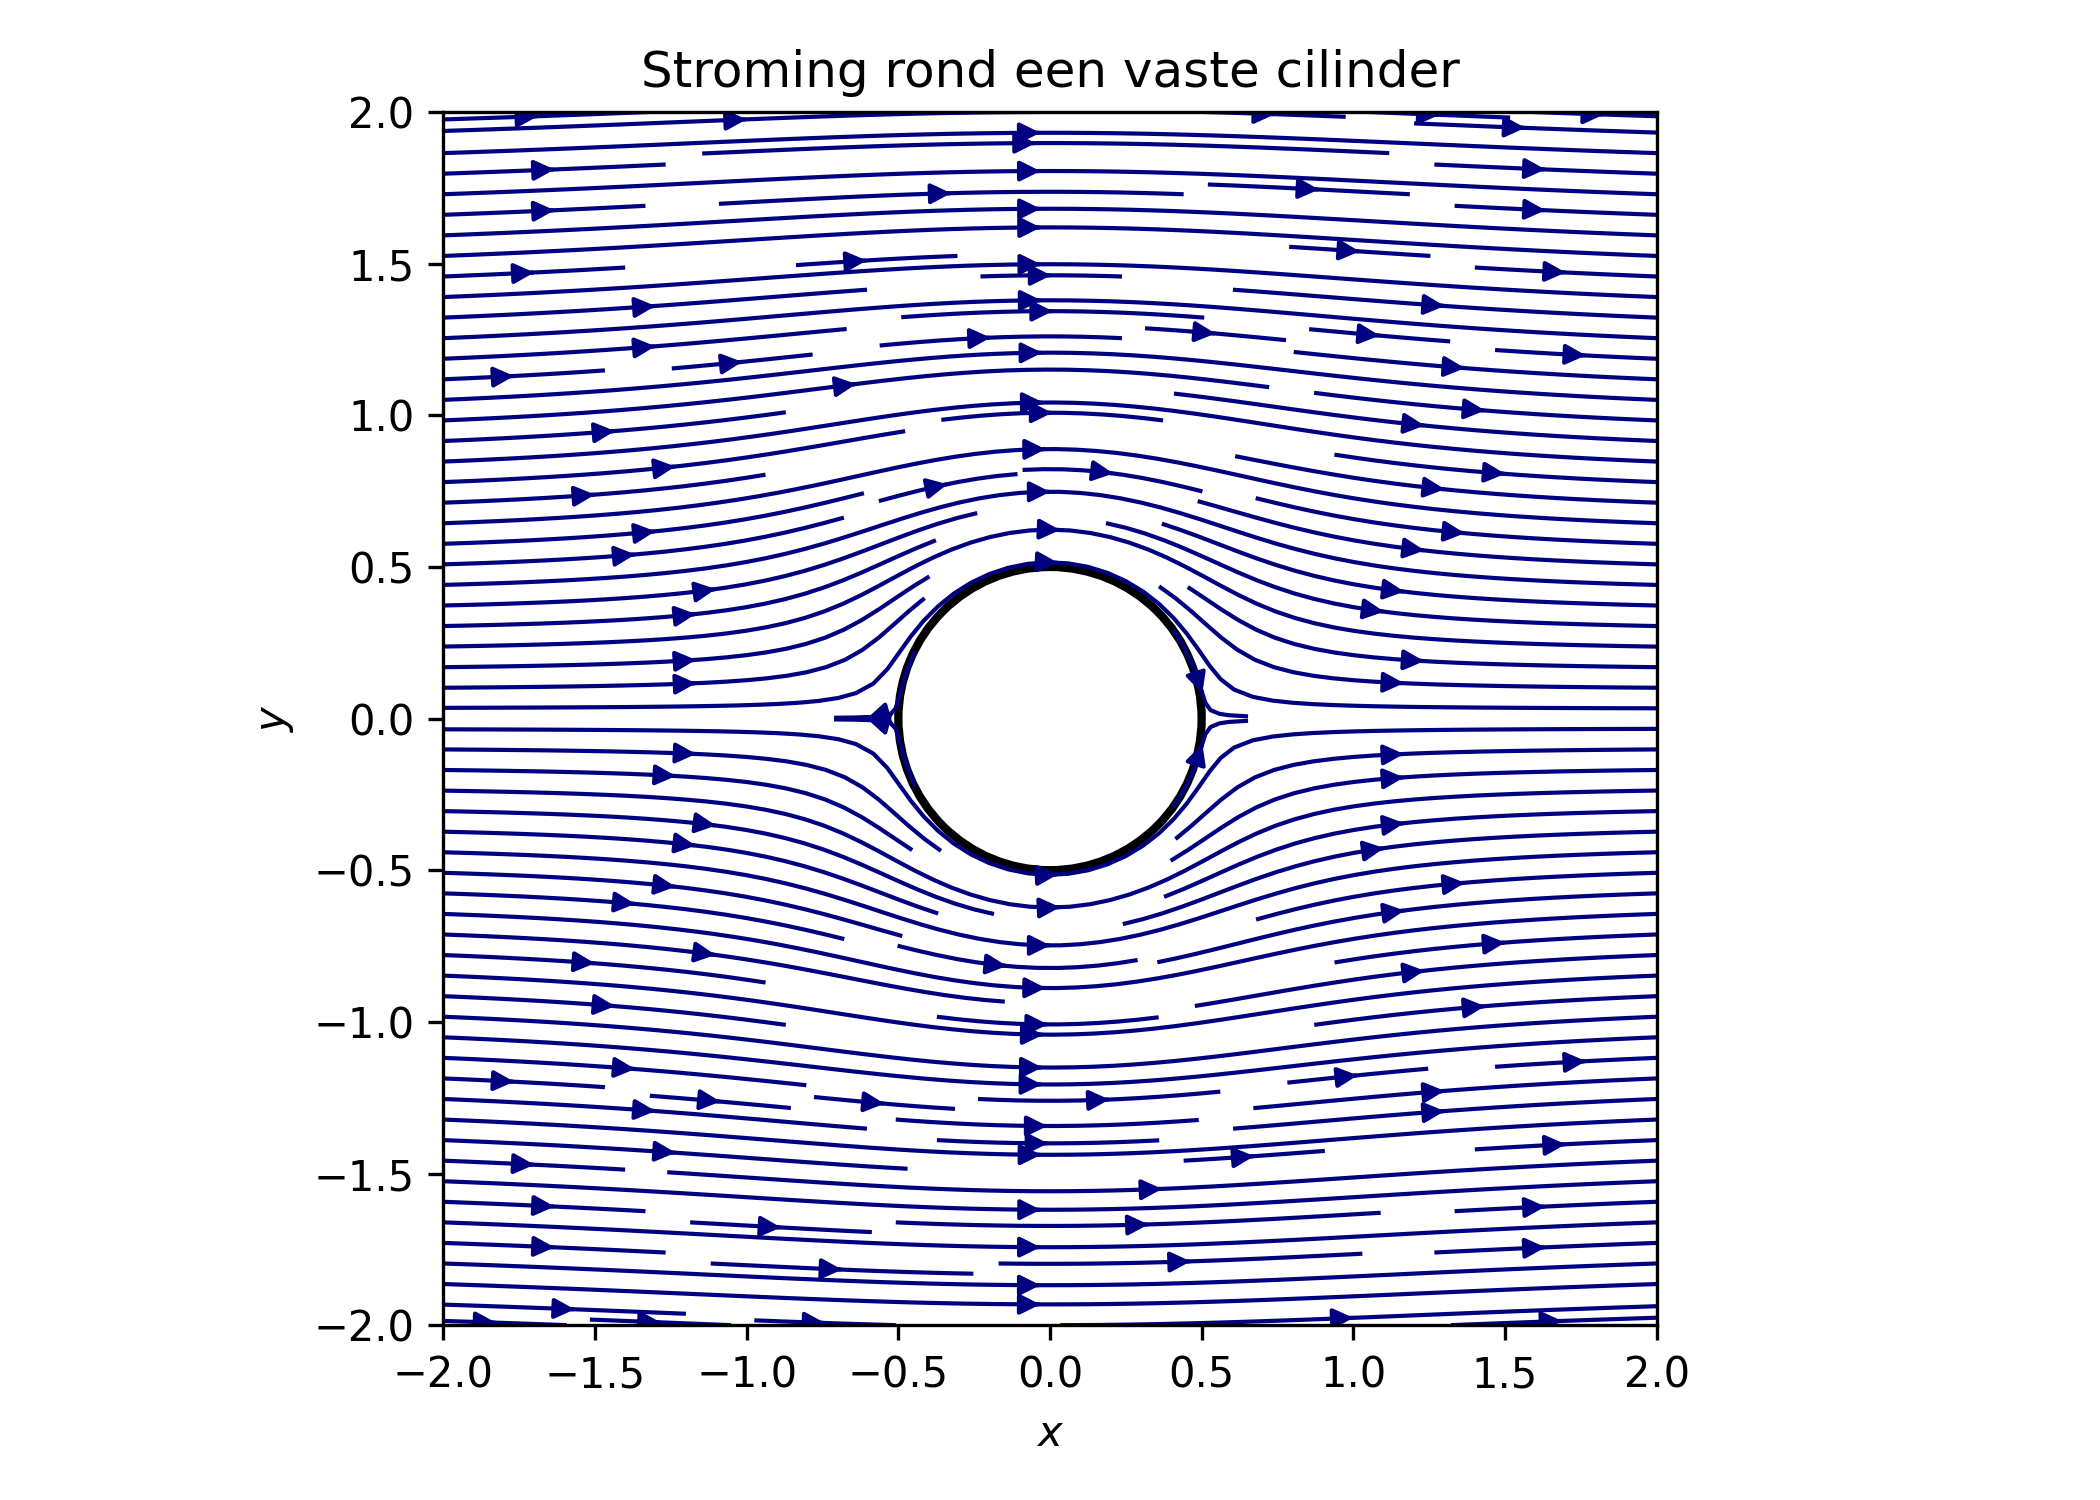
\includegraphics[width=0.85\textwidth]{02_cylinder_stroming}
    \caption{Visualisatie van stroming rond een vaste cilinder als analogie voor ætherstroming rond een stabiele wervel in het æthermodel. De uniforme achtergrondstroom wordt lokaal vervormd door de aanwezigheid van de wervelstructuur. Dit klassieke potentiaalstroomprofiel vormt de basis voor latere interpretaties van ætherinteracties in het model.}
    \label{fig:cylinderflow}
\end{figure}

\section{Introductie}
In een moderne heropleving van Lord Kelvins vortex-atoomhypothese uit 1867~\cite{Kelvin1867-vortex} beschouwen we een absolute Euclidische ruimte gevuld met een supervloeibare ether. Deze hedendaagse etherinterpretatie bouwt voort op en breidt historische kaders uit, zoals de Lorentz-Poincaré-ethertheorie, die absolute kaders en mechanische interpretaties van relativistische verschijnselen introduceerde. In tegenstelling tot deze vroege theorieën integreert het huidige model echter expliciet moderne vloeistofdynamica, topologische vortextheorie en kwantummechanische structuur, waardoor het zich onderscheidt in zowel conceptuele nauwkeurigheid als empirische relevantie. Zo behoudt het de historische continuïteit en biedt het tegelijkertijd een gemoderniseerd en experimenteel verifieerbaar kader.

In dit model worden elementaire deeltjes weergegeven als stabiele vortexknopen of -knooppunten ingebed in de ether, en wordt \emph{tijd} gedefinieerd door de intrinsieke hoekrotatie van hun vortexkernen. De uitdaging is om \emph{tijddilatatie}-wetten af te leiden – analoog aan die in de speciale en algemene relativiteitstheorie (SR en GR) – met behulp van ætherische parameters zoals constante dichtheid, circulatie en Planck-schaaltijd, in plaats van een beroep te doen op 4D-ruimtetijdkromming. We vereisen dat een dergelijke formulering bekende relativistische effecten reproduceert – bijvoorbeeld het vertragen van klokken in de buurt van zware lichamen (gravitationele roodverschuiving) of bij hoge relatieve snelheden (speciaal-relativistische dilatatie) – ondanks dat deze werkt in een vlakke, driedimensionale absolute achtergrond. Met andere woorden, de \emph{werveldynamiek} van de æther – zoals geïllustreerd in figuur ~\ref{fig:cylinderflow} – moet de door kromming veroorzaakte metrische effecten van de algemene relativiteitstheorie met hoge betrouwbaarheid repliceren.

Historisch belangrijke experimenten zoals Michelson-Morley (1887), Pound-Rebka (1959) en Gravity Probe A (1976) bieden indirecte maar consistente ondersteuning voor een ethergebaseerde interpretatie van relativistische verschijnselen. Het Michelson-Morley-experiment legde strenge beperkingen op aan een uniforme etherdrift, terwijl het Pound-Rebka-experiment de door Einstein voorspelde gravitationele roodverschuiving bevestigde. Gravity Probe A bevestigde gravitationele tijdsdilatatie verder met hoge precisie. Deze observaties kunnen op natuurlijke wijze worden geïnterpreteerd binnen het hier gepresenteerde vortex-etherkader, wat zorgt voor empirische coherentie tussen historische en moderne domeinen.

Dit artikel ontwikkelt een wiskundig rigoureus model voor tijdsdilatatie op basis van de dynamiek van vortexrotatie in een onsamendrukbare, niet-viskeuze superfluïde ether. We beginnen met het formaliseren van de fundamentele postulaten van het ethermodel en definiëren hoe de rotatie van een microscopische vortex een fysieke klok vormt. Vervolgens leiden we twee klassen van tijddilatatiewetten af: één voor beweging door de ether (analoog aan SR) en één voor door wervelingen veroorzaakte instromingen rond massa (analoog aan GR). We tonen aan dat deze resultaten kwantitatief standaard relativistische voorspellingen reproduceren – zoals gravitationele roodverschuiving en orbitale klokeffecten – en tegelijkertijd de kromming van de ruimtetijd vervangen door gestructureerde etherstromen en hoeksnelheidsvelden van wervelingen als oorsprong van tijddilatatie.